%==================================================================
%==================================================================
\section{Goodness-of-fit and network comparison}
\frame{\frametitle{Outline} \tableofcontents[currentsection]}
%==================================================================
\frame{\frametitle{Goodness-of-fit (GOF)}

  \paragraph{Aim of GOF tests.} Test if the observed data arise from a given model.

  \medskip
  More cautious: 'if the model fits the data reasonably well'
  
  \bigskip \bigskip \pause
  \paragraph{Typical approach.} 
  \begin{enumerate}
    \setlength{\itemsep}{1.15\baselineskip}
    \item Define some statistic (= function of the data) $T$, 
    \item Establish the distribution of $T$ under the model, 
    \item Compare the observed value of $T$ with its distribution under the model.
  \end{enumerate}

  
  \bigskip \bigskip \pause
  \paragraph{Example.} 
  \begin{enumerate}
    \item Data = observed plant-pollinator network
    \item Statistic $T$ = motif count $N_s$ 
    \item Model = BEDD
  \end{enumerate}

}

%==================================================================
\frame{\frametitle{Goodness-of-fit (GOF) of the BEDD model} \label{sec:GOF}

  \hspace{-.05\textwidth}
  \begin{tabular}{ll}
    \begin{tabular}{p{.5\textwidth}}
      \onslide+<1->{\paragraph{Raw statistic:}
      $$
      T_s = \frac{N_s - \widehat{\Esp} N_s}{\sqrt{\widehat{\Var} N_s}}
      $$ \\ 
      }
      \onslide+<2->{
      \paragraph{Corrected stat.:} accounts for the estimation error in $\widehat{\Esp} N$ \goto{back:GOF}
      $$
      T'_s = \frac{N_s - (\widehat{\Esp} N_s - \emphase{\widehat{\Bias}(\widehat{\Esp} N_s)})}{\sqrt{\emphase{\widehat{\Var} (N_s - \widehat{\Esp} N_s)}}}
      $$ \\ 
      }
%       \onslide+<3>{\paragraph{Choleski\footnote{$\Sigma = P \Lambda P^\intercal$, $\Sigma = P \Lambda^{-1/2} P^\intercal$} transformation:} accounts for the correlation between the counts
%       $$
%       \Sigma_{s, s'} = \Cov(N_s - \widehat{\Esp} N_s, N_{s'} - \widehat{\Esp} N_{s'})
%       $$
%       $$
%       T'' = \emphase{\widehat{\Sigma}^{-1/2}}
%       \left[N_s - (\widehat{\Esp} N_s - \widehat{\Bias}(\widehat{\Esp} N_s))\right]
%       $$
%       }
    \end{tabular}
    &
    \begin{tabular}{p{.4\textwidth}}
      \hspace{-.05\textwidth}
      \onslide+<1->{\paragraph{Zackenberg network.} ~ \\}
      \begin{overprint}
        \onslide<1>
        \includegraphics[width=.4\textwidth]{\fignet/Zackenberg-1996_12-red-StatCount}
        \onslide<2>
        \includegraphics[width=.4\textwidth]{\fignet/Zackenberg-1996_12-red-NormStatCount}
%         \onslide<3>
%         \includegraphics[width=.4\textwidth]{\fignet/Zackenberg-1996_12-red-CholNormStat}
      \end{overprint}
    \end{tabular} 
  \end{tabular}

}

%==================================================================
\frame{\frametitle{Testing degree imbalance}

  \paragraph{Question.} Is there some degree imbalance between plants?
  
  \bigskip \pause
  \paragraph{Statistical test.} 
  \begin{itemize}
    \item Assume $A \sim BEDD(\rho, g, h)$, 
    $$
    \emphase{H_0 = \{h = 1\}}
    $$
    \item For motif $s$, evaluate $\widehat{\Esp}_0(N_s)$ and $\widehat{\Var}_0(N_s)$ and compare 
    $$
    W_s = (N_s - \widehat{\Esp}_0(N_s)) / \sqrt{\widehat{\Var}_0(N_s)}
    $$ 
    with $\Ncal(0, 1)$
  \end{itemize}

  
  \bigskip \pause
  \paragraph{Example.} (only one significant difference) 
  $$
  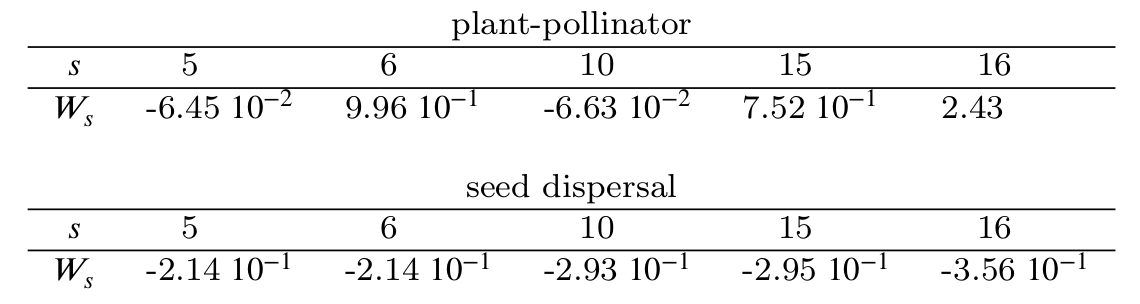
\includegraphics[width=.75\textwidth]{\fignet/OLR22-EJS-Tab3}
  $$
}


%==================================================================
\frame{\frametitle{Comparing network imbalances}

  \bigskip
  \paragraph{Question.} Do network $A$ and $B$ share the same imbalance for pollinators?
  
  \bigskip \pause
  \paragraph{Statistical test.} 
  \begin{itemize}
    \item Assume $A \sim BEDD(\rho^A, g^A, h^A)$ and $B \sim BEDD(\rho^B, g^B, h^B)$
    $$
    H_0 = \{g^A = g^B\}
    $$
    \item For motif $s$, evaluate $\widehat{\Esp}_{\widehat{\rho}^A, \emphase{\widehat{g}^B}, \widehat{g}^A}(N^A_s)$ and $\widehat{\Esp}_{\widehat{\rho}^B, \emphase{\widehat{g}^A}, \widehat{g}^B}(N^B_s)$ and compare 
    $$
    W^{\textcolor{gray}{(g)}}_s\textcolor{gray}{(A, B)} = \frac{(N_s^A - \widehat{\Esp}_0(N_s^A)) - (N_s^B - \widehat{\Esp}_0(N_s^B))}{\sqrt{\widehat{\Var}_0(N^A_s) + \widehat{\Var}_0(N^B_s)}}
    $$ 
    with $\Ncal(0, 1)$
  \end{itemize}

  
  \bigskip \pause
  \paragraph{Example.} (no significant difference) 
  $$
  \begin{array}{c}
    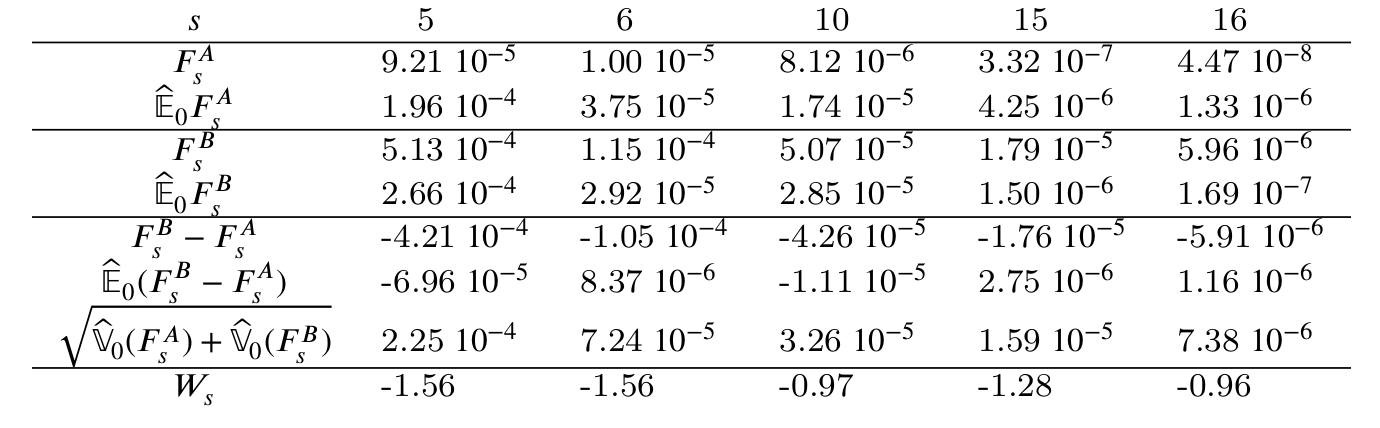
\includegraphics[width=.8\textwidth, trim=0 50 0 0, clip=]{\fignet/OLR22-EJS-Tab4} \\ 
    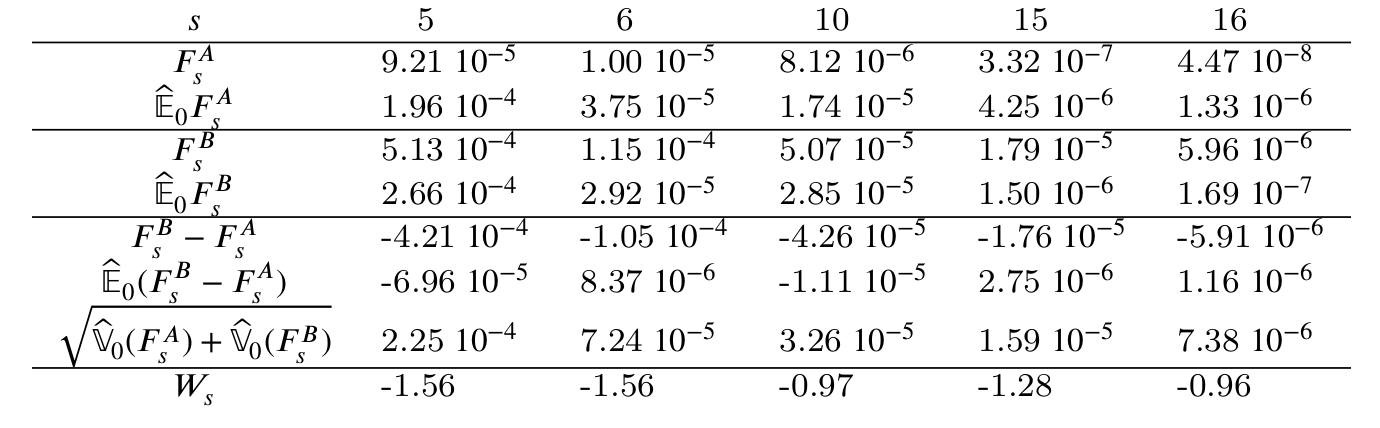
\includegraphics[width=.8\textwidth, trim=0 0 0 90, clip=]{\fignet/OLR22-EJS-Tab4}   
  \end{array}
  $$

}

